% !TEX root = ../ITGO.tex

The welded beam design \citep{WB} is the problem of minimizing the fabrication cost of a welded beam, subject to seven inequality constraints, being two linear and five nonlinear. The constraints include shear stress ($\tau$), bending stress in the beam ($\sigma$), buckling load on the bar ($Pc$), end deflection on the beam ($\delta$) and some more side constraints. The four design variables are continuous. The feasible best known objective value is $f(\bm{x}^*) = 1.7248523$. Figure \ref{fig:WB} presents the schematic of the welded beam design problem. The mathematical formulation of the problem is expressed as follows:

\vspace{-0.5cm}

\begin{align*}
\textbf{Minimize:} & \\
& f(\bm{x}) = 1.10471x_1^2x_2 + 0.04811x_3x_4(14 + x_2) \\[0.5em]
\textbf{subject to:} & \\
& g_1(\bm{x}) = \tau(\bm{x}) - 13,600 \leq 0 \\
& g_2(\bm{x}) = \sigma(\bm{x}) - 30,000 \leq 0 \\
& g_3(\bm{x}) = x_1 - x_4 \leq 0 \\
& g_4(\bm{x}) = 0.10471x_1^2 + 0.04811x_3x_4(14+x_2) - 5  \leq 0 \\
& g_5(\bm{x}) = 0.125 - x_1 \leq 0 \\
& g_6(\bm{x}) = \delta(\bm{x}) - 0.25 \leq 0 \\
& g_7(\bm{x}) = 6,000 - Pc(\bm{x}) \leq 0 \\[0.5em]
\textbf{where:} & \\
& \tau(\bm{x}) = \sqrt{\tau^2 + \frac{(2 \tau' \tau'' x_2)}{2R} + \tau''^2 } \\
& \tau' = \frac{6,000}{(sqrt{2} x_1 x_2)} \\[0.5em]
& \tau'' = \frac{(M R)}{J} \\
& M = 6,000 (14 + \frac{x_2}{2}) \\
& R = sqrt{\frac{x_2^2}{4} + (x_1 + \frac{x_3}{2})^2} \\
& J = 2 x_1 x_2 \sqrt{2} (\frac{x_2^2}{12} + (x_1 + \frac{x_3}{2})^2) \\[0.5em]
& \sigma(\bm{x}) = 504,000 / (x_4 x_3^2) \\
& \delta(\bm{x}) = \frac{65,856,000}{(30 \times 10^6 x_4 x_3^3)} \\
& Pc(\bm{x}) = \frac{4.013(30 \times 10^6)}{196} \sqrt{x_3^2 \frac{x_4^6}{36}} \Bigg(1 - \frac{x_3}{28} \sqrt{\frac{30 \times 10^6}{4(12 \times 10^6)}}\Bigg) \\[0.5em]
\textbf{with bounds:} & \\
&  0.1 \leq x_1, x_4 \leq 2 \\
&  0.1 \leq x_2, x_3 \leq 10
\end{align*}

\vspace{0.5cm}

\begin{figure}[h]
    \begin{center}
    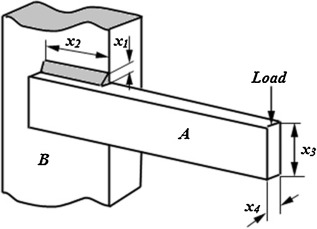
\includegraphics[scale=0.7]{img/Problems/WB.jpg}
    \end{center}
    \captionsetup{justification=centering}
    \caption{Schematic view of the welded beam design problem.}\label{fig:WB}
\end{figure}